\documentclass{article} % Use smaller font size % For LaTeX2e
\usepackage{nips14submit_e,times}
\usepackage[top=0.8in, bottom=0.8in, left=1.0in, right=1.0in]{geometry}
\usepackage{hyperref}
\usepackage{amsmath}
\usepackage{multirow}  % Add this line in the preamble
\usepackage{url}
\usepackage{cite}
\usepackage{graphicx}
\usepackage{subcaption}
%\documentstyle[nips14submit_09,times,art10]{article} % For LaTeX 2.09

\title{Diffusion of Digital Innovations in Heterogeneous Social Networks\\[0.5em]
\large }


\author{
Vinay Joshi\thanks{Alternative Contact: vinaymsjoshi@gmail.com, GitHub:  \url{https://github.com/vinaymsjoshi}} \\
Department of Humanities and Social Sciences\\
Indian Institute of Technology Roorkee\\
Roorkee, Uttarakhand, 247667 \\
\texttt{v\_joshi@hs.iitr.ac.in}
}

\newcommand{\fix}{\marginpar{FIX}}
\newcommand{\new}{\marginpar{NEW}}

\nipsfinalcopy % Uncomment for camera-ready version

\begin{document}

\maketitle

\begin{abstract}
The rapid proliferation of digital innovations, such as digital platforms and online services, has transformed various aspects of modern life. Understanding the mechanisms that drive the adoption of these innovations within diverse social networks is crucial for developers, marketers, and policymakers aiming to enhance user engagement and facilitate widespread diffusion. This study investigates the diffusion dynamics of digital innovations by employing a multi-agent system to simulate individual decision-making processes within heterogeneous social networks. By examining the interplay between network structures, user diversity, payoff gains, and noise levels, this research aims to comprehensively understand how these factors influence rate and stability of innovation diffusion across different network typologies, including random, small-world, and scale-free networks.
\end{abstract}

\section{Introduction}

The diffusion of digital innovations within social networks has been a focal point of research in recent years. The diffusion of digital solutions primarily occurs within user communities, where interactions and communication among individuals play a pivotal role. Since users share information and influence one another, the spread of innovation is largely facilitated by the dynamics of social networks \cite{amini2012alternative, rai2016agent}. Rogers' work on the diffusion of innovations highlights the importance of communication channels and social systems in adoption behaviors \cite{rogers_diffusion_2003}. Granovetter's threshold models further explained how the proportion of adopting peers influences individual adoption decisions \cite{granovetter_threshold_1978}. Additionally, empirical studies have demonstrated that network structures, such as clustering and centrality, significantly impact diffusion patterns \cite{valente_network_1996}. However, there remains a gap in understanding how individual heterogeneity and external factors, like marketing efforts, interact with network structures to affect diffusion outcomes.


This study contributes to the existing literature by integrating user heterogeneity into the diffusion model, categorizing agents into conservative, neutral, and mutable groups, each with distinct decision thresholds. We investigate the diffusion dynamics of such innovations by employing a multi-agent system to simulate the decision-making processes of individual users. Each agent in the network evaluates the benefits of adopting an innovation based on personal preferences, perceived utility, and the influence of connected peers. This approach aligns with findings from agent-based modeling studies that emphasize the importance of capturing individual differences in adoption behaviors \cite{young_diffusion_1996}. Furthermore, this research examines the impact of network effects, both local and global, on diffusion dynamics. Prior studies have shown that network effects can accelerate adoption and sustain diffusion by reinforcing the perceived value of the innovation within the community \cite{muller_network_2019}. Some studies indicated the presence of network effects in the diffusion of mobile applications in the real world, where the utility derived by users increases as the number of adopters grows \cite{song2018ecosystem}. This study provides insights into optimizing diffusion strategies by analyzing how varying network structures provided in Figure 1 influence these effects.

\begin{figure}[h]
    \centering
    \begin{subfigure}{0.2\textwidth}
        \centering
        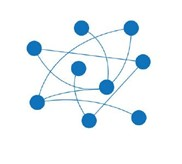
\includegraphics[width=\linewidth]{1111111.jpg} % Replace with actual path
        \caption{Random}
        \label{fig:random_network}
    \end{subfigure}%
    \hspace{0.05\textwidth} % Adjusts spacing between images
    \begin{subfigure}{0.205\textwidth}
        \centering
        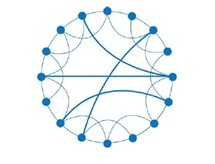
\includegraphics[width=\linewidth]{2222222.jpg} % Replace with actual path
        \caption{Small-World}
        \label{fig:small_world_network}
    \end{subfigure}%
    \hspace{0.05\textwidth} % Adjusts spacing between images
    \begin{subfigure}{0.2\textwidth}
        \centering
        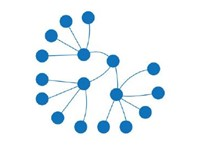
\includegraphics[width=\linewidth]{3333333.jpg} % Replace with actual path
        \caption{Scale-Free}
        \label{fig:scale_free_network}
    \end{subfigure}
    \caption{Different Network Structures}
    \label{fig:network_structures}
\end{figure}


Moreover, this research incorporates the role of noise in decision-making processes, acknowledging that random factors often influence real-world choices. Studies on social learning suggest that noise can both facilitate and disrupt diffusion, depending on user susceptibility and network structure \cite{young_individual_1998}. By simulating different noise levels, this study explores their impact on adoption rates and the formation of stable adoption clusters.

The current study investigates the diffusion of digital solutions from individual users to broader user groups. Using agent-based modeling techniques \cite{jiang2020review, yi2018management}, which enable the exploration of user behavior at a granular level, this research develops a simulation framework to model individual decision-making and the intricate interactions among users within social networks. Specifically, the study focuses on the following: (i) analyzing user behavior characteristics to identify key factors influencing decision-making, establishing a conceptual framework for adoption and rejection decisions, using social learning methods to depict decision-making processes and interactions within heterogeneous social networks; (ii) conducting multi-agent simulations to explore the diffusion of mobile applications across various network structures and network effects; and (iii) examining the influence of network effects and firm promotional strategies on diffusion through simulation experiments, emphasizing the role of user personality traits and the influence of neighbors on personal decision-making, presenting practical recommendations for firms to enhance promotion strategies and optimize the diffusion of mobile applications.

\section{Methodology}

The model framework includes developing a multi-agent system, where each user in the network is represented as an autonomous agent with distinct characteristics. This setup simulates the diffusion of digital innovations—such as new software platforms, smartphone apps, or online services—within social networks having heterogeneous user behavior and network structures. The model aims to capture the decision-making processes of individual users who interact with their neighbors and adopt or reject the innovation based on personal preferences, perceived benefits, and influence from connected peers. 

\subsection{Designing the Conceptual Framework}

We start by outlining the assumptions regarding adopting digital innovations within the user community. Next, we develop a model based on an analysis of user behavior characteristics and the factors influencing their decision-making processes. 

\subsubsection{Assumptions for Innovation Diffusion}

The foundational assumptions of models play a crucial role in simulating user decision-making processes. Based on previous studies \cite{bryson2007agent, joseph2020organizational}, we establish the following assumptions regarding individual decision-making behavior, consumer attributes, and the characteristics of the digital innovation being studied:

\begin{enumerate}
    \item The digital innovation under consideration serves as a generalized representation of common attributes and features,  typically associated with digital platforms in the market. Any modifications to platform features during the diffusion process are disregarded.
    \item The diffusion of the chosen digital platform is considered in isolation, assuming it is unaffected by the presence of competing platforms. Thus, our model focuses solely on the spread of a single innovation within the user network.
    \item Users obtain information about the platform’s utility and decision-making context through interactions with their social connections. Due to information processing limitations, users cannot make predictions for the long term.
    \item When presented with the same platform, users may make different decisions based on individual preferences and personality traits, highlighting variability in decision-making behavior. 
    \item Users acquire information about digital platforms primarily through public media and advertisements, and social influence, where opinions are shared within their network. Based on information processing theory, individual decisions are influenced by external environmental information and personal preferences and attitudes toward decision-making \cite{hann2007overcoming}.



 
\end{enumerate}

We developed a model where users assess the perceived utility of the platform by considering benefits, costs, and network effects. Additionally, they also consider neighborhood influence, and then, based on this information and individual traits, users choose to adopt or reject the platform. 

\subsubsection{User Decision-Making and Interaction Process}

Based on the assumptions for the diffusion of digital applications, we have designed an interaction process between the individual agents, along with the decision-making process they finally use to decide whether to adopt the innovation or stick with the status quo. Initially, the current value of the digital platform is assessed from the user’s decision-making perspective. Next, the information on neighboring users' choices is gathered. Additionally, user preferences, personality traits, and interactions with their network play a role in influencing decisions. 

By evaluating the platform's utility, users decide whether to adopt or reject it in subsequent steps. During the diffusion process, individuals can communicate with other users and game theory is frequently applied to model these interactions between individuals \cite{ozkan2016evolutionary, zhang2019competitive}. Consequently, we also utilize a game-theoretic matrix to represent user interactions, as depicted in Table 1.

\begin{table}[h]
\caption{Game matrix of user decision-making behavior.}
\label{game-matrix}
\begin{center}
% Set a general arraystretch for the whole table
\renewcommand{\arraystretch}{1.5}
\begin{tabular}{c c c}
    \hline
    \textbf{User 1} & \multicolumn{2}{c}{\textbf{User 2}} \\ \cline{2-3}
    & Adopt & Reject \\
    \hline
    Adopt & $b - c + \frac{m}{n \cdot k}, b - c + \frac{m}{n \cdot k}$ & $b - c + \frac{m}{n \cdot k}, b - f$ \\
    % Temporarily reduce arraystretch for compact rows
    \renewcommand{\arraystretch}{1.5}
    Reject & $b - f, b - c + \frac{m}{n \cdot k}$ & $0, 0$ \\
    \hline
\end{tabular}
% Reset arraystretch to default
\renewcommand{\arraystretch}{1}
\end{center}
\end{table}
In the above game matrix, \( b \) denotes the utility value derived from the digital innovation, \( c \) represents the usage cost associated with it, and \( f \) reflects the benefit loss incurred when a user decides to reject the innovation. If a user chooses to reject the digital product, they receive a net return of \( b - f \), where \( b > f \). Additionally, \( n \) is the total user population, while \( m \) represents the investment in promotion and marketing by companies. The term \( \frac{m}{n \cdot k} \) captures the value each user gains from corporate marketing efforts when they adopt the application. We assume that within each fixed time step, \( k \) denotes the percentage of users adopting the digital solution. Using these interpretations, the expected benefits for a user in the case of adoption and rejection are calculated, respectively:

\begin{equation}
E_A = \left( b - c + \frac{m}{n \cdot k} \right) \cdot k + \left( b - c + \frac{m}{n \cdot k} \right) \cdot (1 - k) = b - c + \frac{m}{n \cdot k}
\end{equation}

\begin{equation}
E_B = (b - f) \cdot k + 0 \cdot (1 - k) = (b - f) \cdot k
\end{equation}

When some individuals in the user network adopt the innovation (i.e., \( k > 0 \)), the revenue from adoption becomes \( b - c + \frac{m}{n \cdot k} \), while the revenue from rejection stands at \( (b - f) \cdot k \). If no users adopt the application, the benefit is zero. 

The utility value influencing a user’s decision-making is influenced by three key components: (i) the anticipated benefit from the innovative solution (\( E_i \)), (ii) individual user preferences (\( \text{pre}_i \)), and (iii) the network effect (\(d \cdot D_i(t - 1) \)). Consequently, the utility for user \( i \) to either adopt or reject the digital innovation at time \( T \) can be expressed as:

\begin{equation}
U_i(t) = E_i + \text{pre}_i + d \cdot D_i(t - 1)
\end{equation}

Here, \( E_i \) denotes the expected gains for user \( i \), \( d \) signifies the network utility of the application (measure of network effect intensity), and \( \text{pre}_i \) represents the user's personal preference. \( D_i(t - 1) \) is defined to represent the utility derived from different types of network effects. 

In a \textbf{global network context}, \( D_i(t - 1) = k \) at time \( t - 1 \), indicating the proportion of users who adopted the application. In a \textbf{local network context}, \( N_i(t - 1) \) represents the number of neighboring users who adopted the application at \( t - 1 \), and \( z_i \) denotes the degree (number of connections) of user \( i \). Thus, \( D_i(t - 1) = \frac{N_i(t - 1)}{z_i} \). The final utilities for adopting digital innovation in global and local network effects are depicted by expressions (4) and (5), respectively. 

\begin{equation}
U_a = b - c + \frac{m}{n \cdot k} + \text{pre}_i + d \cdot k
\end{equation}

\begin{equation}
U_a = b - c + \frac{m}{n \cdot k} + \text{pre}_i + d \cdot \frac{N_i(t - 1)}{z_i}
\end{equation}

If a user chooses to reject the digital innovation, they let go of the network benefits. The utility function for the rejection strategy at time \( t \) in both types of network effects is defined as:

\begin{equation}
U_b = (b - f) \cdot k + \text{pre}_i
\end{equation}

\textit{\textbf{Heterogeneity in Population}}: Users are classified based on their decision-making approach in the context of innovation adoption, resulting in three categories: \textbf{conservative}, \textbf{neutral}, and \textbf{mutable}, denoted by \( P_c \), \( P_n \), and \( P_m \). Each category of users follows distinct probability distributions for determining their decision thresholds, with \( P_c \sim \text{Uniform}(0.7, 1) \), \( P_n \sim \text{Uniform}(0.4, 0.7) \), and \( P_m \sim \text{Uniform}(0, 0.4) \), respectively.

Unlike diffusion in traditional networks, in our diffusion model, the individual’s decision-making process is influenced by both personal preferences and neighbors' choices, while communication and interaction within the social network also impact decisions. To capture this, we apply a \textbf{social learning mechanism}, facilitating user interactions. Also, the heterogeneity in the user base should be considered while learning decision-making behaviors from neighbors. Users with similar decision attitudes are likelier to imitate each other, while those with differing traits are less likely to adopt the same decision. We define separate imitation probabilities for different pairs of user types. The matching probability between individuals \( a \) and \( b \) with respective attitudes \( P_a \) and \( P_b \) is represented by \( \text{Match}(P_a, P_b) \in (0, 1) \), where \( a, b \in \{c, n, m\} \). The specific mappings are as follows: \( \text{Match}(P_c, P_c) = \text{Uniform}(0.7, 1) \), \( \text{Match}(P_c, P_n) = \text{Uniform}(0.4, 0.7) \), \( \text{Match}(P_c, P_m) = \text{Uniform}(0, 0.4) \), \( \text{Match}(P_n, P_n) = \text{Uniform}(0.7, 1) \), \( \text{Match}(P_n, P_m) = \text{Uniform}(0.4, 0.7) \), and \( \text{Match}(P_m, P_m) = \text{Uniform}(0.7, 1) \).

\textit{\textbf{Social Influence Theory}}: Users compare their own utility with that of their neighbors. If a user’s utility value is greater than those of all their neighbors, they will continue with their current decision in the next step. However, if a neighbor’s utility exceeds their own, the user will adopt the decision-making strategy of the neighbor with the highest utility, with a probability given by the below expression:

\begin{equation}
P = \frac{1}{1 + e^{-\frac{(U_j - U_i)}{r}}}
\end{equation}

where \( U_i \) represents the user’s utility from the digital innovation, \( U_j \) is the utility of the neighbor being observed, and \( r \) denotes the noise in the social learning process. If the decision-learning probability given by equation (7) surpasses the defined matching threshold, the user adopts the neighbor's decision. Otherwise, the matching threshold is compared with the individual decision threshold, and the user maintains their current decision if the matching probability is less than the user decision threshold. When successful in imitating a neighbor's decision, the user preserves this strategy in the subsequent time step. In the further time steps, the users may adjust their decision state again following the same social learning process. Thus, the iterative process allows the agents to continuously interact and update their decisions based on perceived benefits and differences in decision states.

\subsubsection{Modelling Processes}
The simulation framework allows for specifying the initial interaction graph among the user agents. Each user agent in the network is treated as an object with distinct properties and two possible states: adopt or reject. The initial state includes a subset of users randomly designated as initial adopters or "seed" users. Next, the utilities are calculated for each user according to their own and their neighbors' decision state. Then, each agent's decision-making and interaction mechanisms in the user network are implemented. Finally, the multi-agent model simulates diffusion of digital innovation, incorporating social network effects, where the population freely interacts among themselves according to the conceptual model designed. The process steps are summarized in Table 2.
\begin{table}[h]
\caption{Process of our simulation model.}
\label{simulation-model}
\begin{center}
\renewcommand{\arraystretch}{1.3} % Adjust row height
\vspace{-0.5em} % Reduce space above the table
\begin{tabular}{p{14cm}}
    \hline
    \textbf{Model 1. Simulation of User Decisions about Innovative Digital Solutions Using Multi-Agents} \\ \hline
    \textbf{Input:} Agent and the parameters \( b, c, m, n, \textit{prei} \), social networks structure \textit{network\_type} \\
    \textbf{Output:} All user decisions \textit{user\_states(t)} \\ \hline
    \textbf{1.} Initialize Agent, build different social networks \\
    \textbf{2.} \textbf{for} \( t \) in times \( T \): \\
    \hspace{0.5cm} $\bullet$ utility calculation for each agent in \( t \); // Equations (4), (5), and (6) \\
    \hspace{0.5cm} $\bullet$ agents interact and learning happens among users and their neighbors; // Equation (7) \\
    \hspace{0.5cm} $\bullet$ simulate user’s decision-making process concerning innovation; capture in // \textit{user\_states(t)} \\
    \hspace{0.5cm} $\bullet$ collect statistics on user decisions and create visualizations at \( t \); \\
    \textbf{3.} \textbf{end-loop} \\
    \textbf{4.} return \textit{user\_states(t)} \\ \hline
\end{tabular}
\vspace{-1em} % Reduce space below the table
\end{center}
\end{table}

The parameters and variables within each \texttt{user} agent are structured to support decision-making and interaction processes in the context of the digital solution's diffusion. Key parameters include \texttt{Cht}, which represents the personality of a user, where \( \texttt{Cht} = \{1, 2, 3\} \) corresponds to conservative, balanced, and mutable behaviors, respectively; \texttt{Pre}, indicating user preference towards the platform, which follows a normal distribution \( N(\mu, \sigma) \); \texttt{user\_state}, a Boolean parameter that specifies whether a user adopts or rejects the platform at time \( t \); \texttt{stickiness}, which induces stickiness to the user decision, once the user imitates one of its neighbors; \texttt{ra1} and \texttt{ra2}, which are the probabilities of state change after adoption and rejection, respectively; \texttt{k\_local}, denoting the fraction of neighboring users who adopt the platform, contributing to the local network effect; and \texttt{user\_degree}, representing the number of neighbors or the user's degree within the social network.
\section{Analysis and Results}

In this section, we analyze the diffusion patterns of digital innovations within various social network configurations, examining the roles of user distributions, network structures, and network effects. Using the simulation framework established in the methodology, we evaluate how different network characteristics influence the adoption and spread of digital solutions. This analysis encompasses the impact of network effect intensity, payoff gains, noise levels, and other key parameters on diffusion dynamics. The simulations were run multiple times, with the average number of adopters calculated across iterations to ensure robustness in the interpretation.

\subsection{Diffusion Dynamics Across Diverse User Distributions}

\begin{figure}[h]
    \centering
    % First row of subfigures
    \begin{subfigure}{0.3\textwidth}
        \centering
        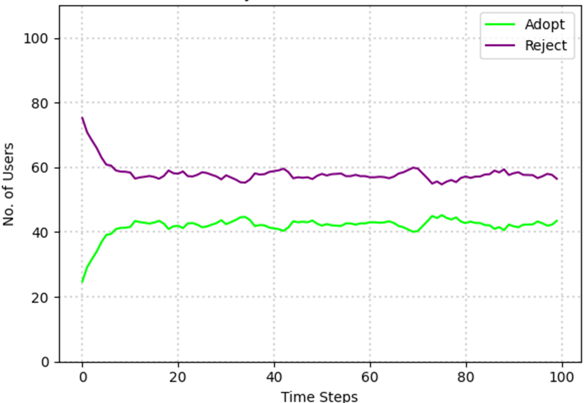
\includegraphics[width=\linewidth]{1.png} % Replace with the actual path
        \caption{}
        \label{fig:subfig_a}
    \end{subfigure}
    \hspace{0.05\textwidth} % Adjusts spacing between images
    \begin{subfigure}{0.3\textwidth}
        \centering
        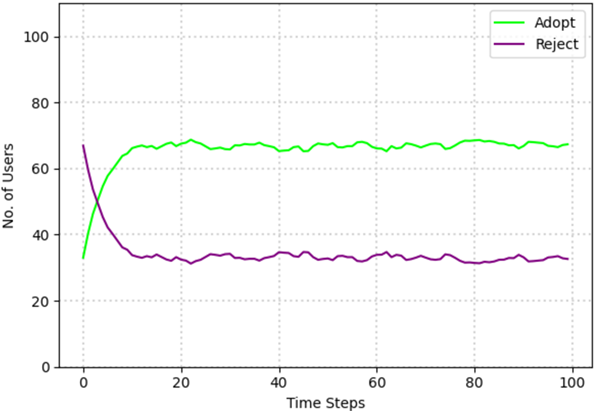
\includegraphics[width=\linewidth]{2.png} % Replace with the actual path
        \caption{}
        \label{fig:subfig_b}
    \end{subfigure}
    
    % Second row of subfigures
    \vspace{0.5cm} % Space between rows
    \begin{subfigure}{0.3\textwidth}
        \centering
        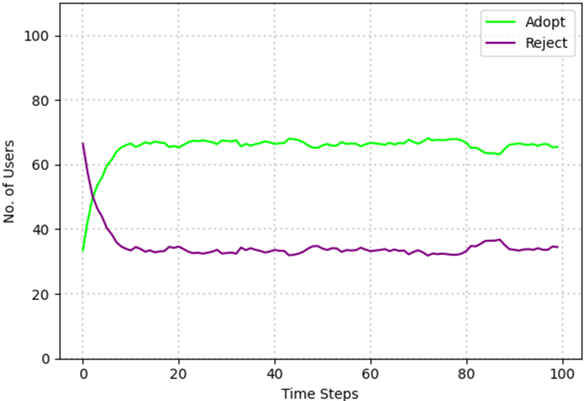
\includegraphics[width=\linewidth]{3.png} % Replace with the actual path
        \caption{}
        \label{fig:subfig_c}
    \end{subfigure}
    \hspace{0.05\textwidth} % Adjusts spacing between images
    \begin{subfigure}{0.3\textwidth}
        \centering
        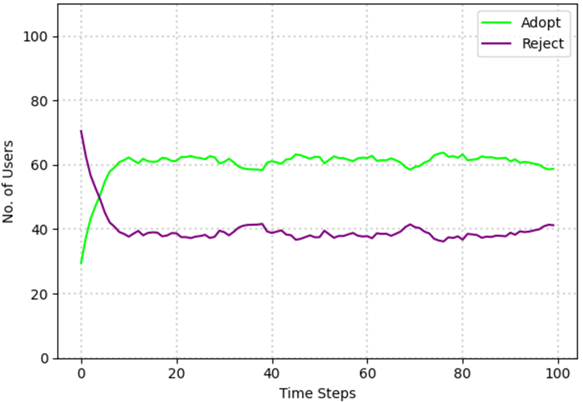
\includegraphics[width=\linewidth]{4.png} % Replace with the actual path
        \caption{}
        \label{fig:subfig_d}
    \end{subfigure}
    
    \caption{(a) Conservative users only, \( \phi_{Cht} = (1, 0, 0) \); (b) Mutable users only, \( \phi_{Cht} = (0, 0, 1) \); (c) Balanced users only, \( \phi_{Cht} = (0, 1, 0) \); and (d) Mixed distribution, \( \phi_{Cht} = (0.3, 0.3, 0.4) \).}
    \label{fig:diffusion_dynamics}
\end{figure}
The simulations are performed having four different user preference distributions: \( \phi_{Cht} = (1, 0, 0) \). (b) \( \phi_{Cht} = (0, 0, 1) \). (c) \( \phi_{Cht} = (0, 1, 0) \). (d) \( \phi_{Cht} = (0.3, 0.3, 0.4) \). \( \phi_{Cht}(C,N,M)\) is used to denote the percentage of conservative, neutral and mutable users in the population. The model is initialized with 100 users in a random network and we ran it for 100 time steps. Seed users constituted 20\% of the total population. The utility parameters for the digital innovation in the simulation were set as follows: \( b = 100 \), \( C = 85 \), \( f = 35 \), and \( M = 0 \), while the network effect intensity, \( d \), was assigned a value of 30. 

In Figure 2(a), the conservative users maintain a stable adoption rate, showing little change in decisions due to lower susceptibility to influence. As a result of the resistance of the conservative users, the number of adopters for the innovation end up being less than the rejectors. In contrast, Figure 2(b) demonstrates that mutable users frequently shift their decisions, reflecting their responsiveness to social influences. The adopters rapidly increase in the population, owing to the mutable nature of the agents. As depicted in Figure 2(c), balanced users exhibit moderate variability, and have relatively higher innovation diffusion than purely conservative network. Finally, Figure 2(d) shows a distribution with 30\% conservative, 30\% balanced, and 40\% mutable users. When adoption level reaches a certain threshold, the variability within the user group diminishes, indicating a stable diffusion state for the innovation in the market. The final diffusion level is lower than in purely mutable or purely balanced user scenarios, which is because to the existence of some conservative users.

Comparing these simulation outcomes to real-world behavior reveals consistent results, confirming the model's reliability and robustness for analyzing the diffusion of digital innovations in heterogeneous social networks.

\subsection{Diffusion Dynamics Across Different Network Structures and Effects}

This section analyzes how diffusion dynamics change in different types of social networks: random networks, small-world networks, and scale-free networks. We also used different network effects: global network effect and local network effect, to study their influence on the diffusion process. Each experiment was repeated 50 times, with the results averaged to ensure consistency.

The simulations are configured with a total of 100 users, an average network degree of 6, and individual user preferences distributed as \( Pre \sim N(50, 10) \). For all trials, the user preference distribution was kept at \( \phi_{Cht} = (0.3, 0.3, 0.4) \), with parameters \( b = 120 \), \( c = 105 \), \( f = 55 \), and \( m = 0 \), over a duration of 100 time steps. We separately analyze the diffusion for random, small-world and scale-free network structures, under the two network effects.
\begin{figure}[h]
    \centering
    % First row of subfigures
    \begin{subfigure}{0.3\textwidth}
        \centering
        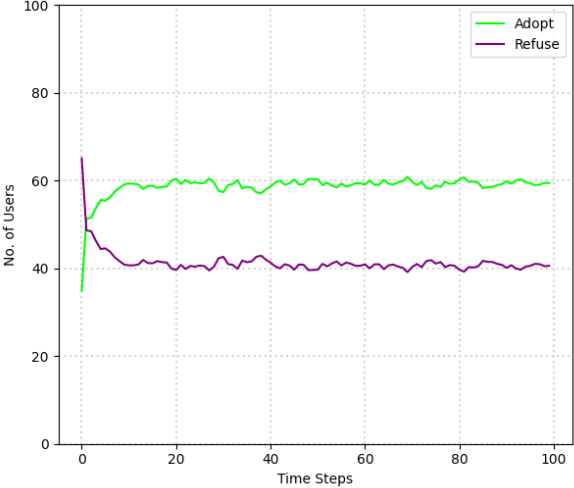
\includegraphics[width=\linewidth]{11.png} % Replace with the actual path
        \caption{}
        \label{fig:subfig_a}
    \end{subfigure}
    \hspace{0.02\textwidth} % Adjusts spacing between images
    \begin{subfigure}{0.3\textwidth}
        \centering
        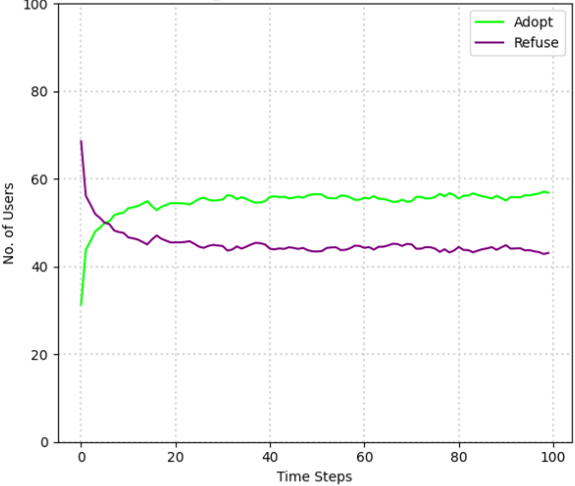
\includegraphics[width=\linewidth]{22.png} % Replace with the actual path
        \caption{}
        \label{fig:subfig_b}
    \end{subfigure}
    \hspace{0.02\textwidth} % Adjusts spacing between images
    \begin{subfigure}{0.3\textwidth}
        \centering
        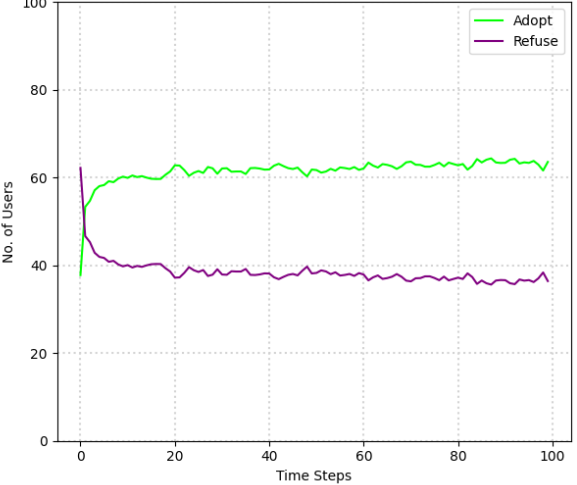
\includegraphics[width=\linewidth]{33.png} % Replace with the actual path
        \caption{}
        \label{fig:subfig_c}
    \end{subfigure}
    
    % Second row of subfigures
    \vspace{0.5cm} % Space between rows
    \begin{subfigure}{0.3\textwidth}
        \centering
        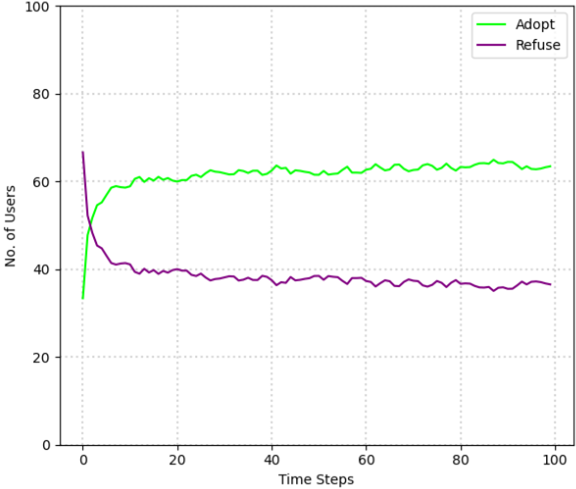
\includegraphics[width=\linewidth]{44.png} % Replace with the actual path
        \caption{}
        \label{fig:subfig_d}
    \end{subfigure}
    \hspace{0.02\textwidth} % Adjusts spacing between images
    \begin{subfigure}{0.3\textwidth}
        \centering
        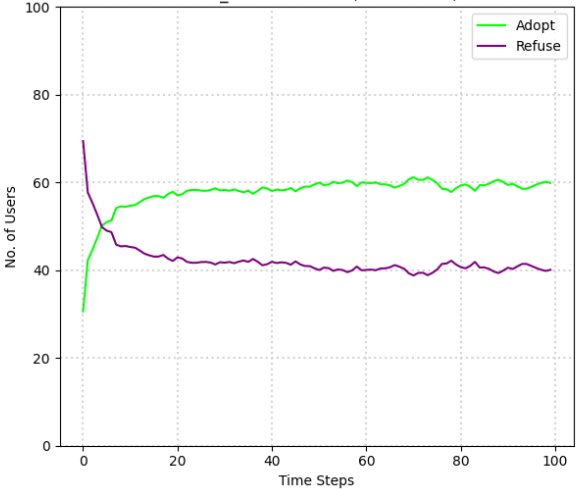
\includegraphics[width=\linewidth]{55.png} % Replace with the actual path
        \caption{}
        \label{fig:subfig_e}
    \end{subfigure}
    \hspace{0.02\textwidth} % Adjusts spacing between images
    \begin{subfigure}{0.3\textwidth}
        \centering
        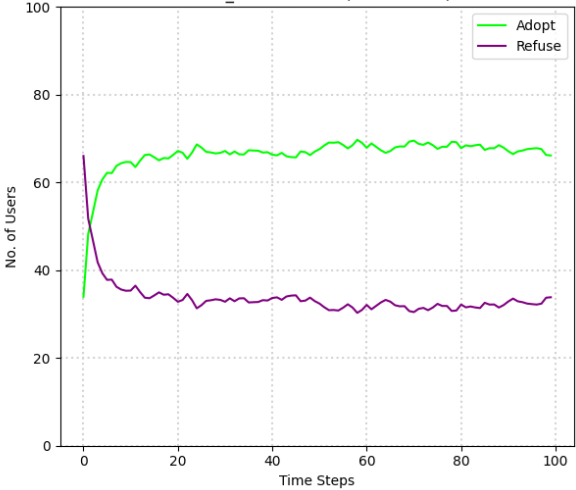
\includegraphics[width=\linewidth]{66.png} % Replace with the actual path
        \caption{}
        \label{fig:subfig_f}
    \end{subfigure}
    
    \caption{(a) Random network with global network effect; (b) Small-world network with global network effect; (c) Scale-free network with global network effect; (d) Random network with local network effect; (e) Small-world network with local network effect; and (f) Scale-free network with local network effect.}
    \label{fig:network_dynamics}
\end{figure}

\subsubsection{Diffusion under the Global Network Effect}

Figure 3(a)-(c) illustrates the diffusion patterns under the global network effect for random, small-world, and scale-free networks. Across all network structures, diffusion begins with a slow initial increase, followed by a wave-like decline before stabilizing. In terms of speed, both random and scale-free networks exhibit similar diffusion rates, with group decisions reaching equilibrium faster than in small-world networks. This rapid adoption is due to frequent social interactions and the reinforcing influence of network effects. Notably, adoption within small-world networks progresses more slowly, and final adoption levels remain lower than in the other two networks.

Comparing network structures, scale-free networks achieve the highest adoption rate, followed by random networks, with small-world networks lagging. Scale-free networks benefit from central hub nodes that facilitate value propagation, enabling these influential nodes to promote innovation by spreading utility information through extensive social ties. This configuration allows hub nodes to affect the decision-making of neighboring users swiftly, amplifying adoption within the network. Consequently, the scale-free structure achieves the most effective diffusion under global network effects.

\subsubsection{Diffusion under the Local Network Effect}

The simulations under local network effects, as shown in Figures 3(d)–(f), indicate similar adoption trends across the three network structures. However, under the local effect, diffusion within scale-free networks becomes more pronounced compared to random or small-world networks. This is because users in small-world networks experience highly localized interactions with similar utility values, making it challenging for diffusion to propagate across different small groups. As a result, adoption remains concentrated within individual clusters.

Under the local network effect, the scale-free network demonstrates the highest adoption rate, followed by random and small-world networks. The limited diffusion within small-world networks arises from the difficulty of transmitting adoption momentum across clusters. Conversely, the scale-free network’s hubs enable stronger localized diffusion, as these influential nodes increase the perceived utility of the innovation within their social circles. This setup amplifies the role of social learning, making the scale-free structure the most suitable for diffusion under local network effects.

The comparison of results under global and local network effects reveals that local effects generally enhance adoption rates, as users are more influenced by neighboring adopters. This highlights the role of immediate social surroundings in reinforcing adoption decisions. This dynamic underlines that local network effects create more robust diffusion outcomes than global effects, particularly in networks with high centrality nodes.

\subsection{Sensitivity Analysis of Different Network Parameters}

\subsubsection{Network Effect Intensity}

We implement simulations to explore the effect of increasing network intensity on spread of innovation within a user community. The parameters used in this model were set as follows: \( B = 130 \), \( C = 110 \), \( f = 55 \), and \( M = 0 \). The outcomes of the simulation are presented in Figure 4.
\begin{figure}[h]
    \centering
    % Subfigure (a)
    \begin{subfigure}{0.42\textwidth}
        \centering
        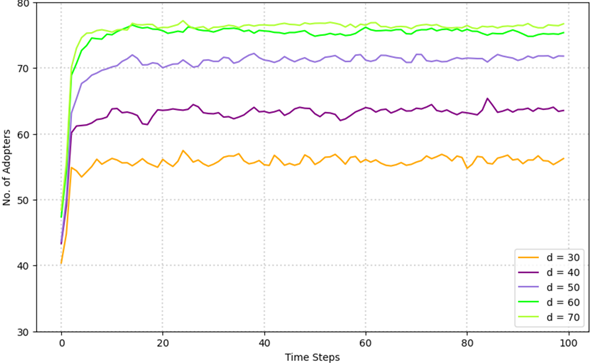
\includegraphics[width=\linewidth]{111.png} % Replace with the actual path
        \caption{}
        \label{fig:sensitivity_global}
    \end{subfigure}
    \hspace{0.05\textwidth} % Adjusts spacing between images
    % Subfigure (b)
    \begin{subfigure}{0.42\textwidth}
        \centering
        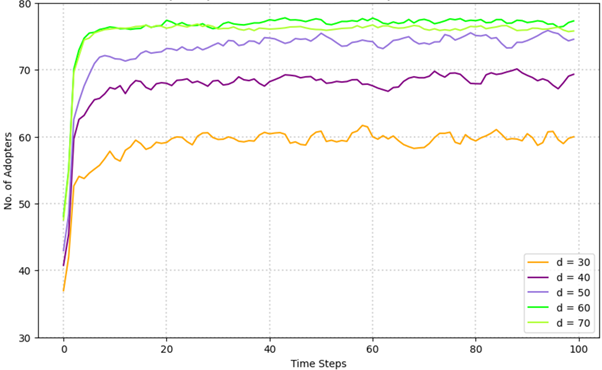
\includegraphics[width=\linewidth]{222.png} % Replace with the actual path
        \caption{}
        \label{fig:sensitivity_local}
    \end{subfigure}
    
    \caption{(a) Sensitivity analysis under the global network effect (\( d = 30, 40, 50, 60 \)). (b) Sensitivity analysis under the local network effect (\( d = 30, 40, 50, 60 \)).}
    \label{fig:sensitivity_analysis}
\end{figure}
The simulation results using random network highlights that a higher network effect intensity leads to broader adoption of innovation across the network, thereby enhancing overall diffusion. As the intensity of the network effect rises, the perceived utility of the innovation increases among users. Consequently, even individuals who initially opted not to adopt the application may reconsider due to the influence of social learning, leading to a gradual increase in adopters. The mutual reinforcement between the number of adopters and the network effect increases the adoption process, ultimately resulting in more effective diffusion outcomes. Conversely, when the network effect intensity is low, the diffusion is slower, and the influence of additional users is limited, making it difficult to significantly increase the overall adoption rate.

Comparing the global and local network effects, we observe that under local network effects, diffusion tends to proceed more rapidly, even with the same network intensity level, especially in the initial stages of the diffusion process. This suggests that local network effects have a stronger immediate influence on diffusion speed than global effects, which can be observed through larger adoption rates in the case of local network effect, when d = 30, 40. However, as d increases, nearly similar diffusion rates are observed in both scenarios. This is intuitive, because increase in d value means that even distant users feel the impact of adopters more strongly, which accelerates diffusion throughout the entire network. This increased reach diminishes the unique advantage of local effects, where immediate social circles initially drive adoption. 

\subsubsection{Innovation Diffusion under Company Marketing and Promotion}
The marketing promotion parameter is adjusted to conduct a sensitivity analysis, with values of \( m = 10 \), \( m = 20 \), and \( m = 30 \) for comparison. The other parameters in the model were set to \( B = 130 \), \( C = 120 \), and \( f = 55 \), with the proportion of initial adopters set at 10\%. 
\begin{figure}[h]
    \centering
    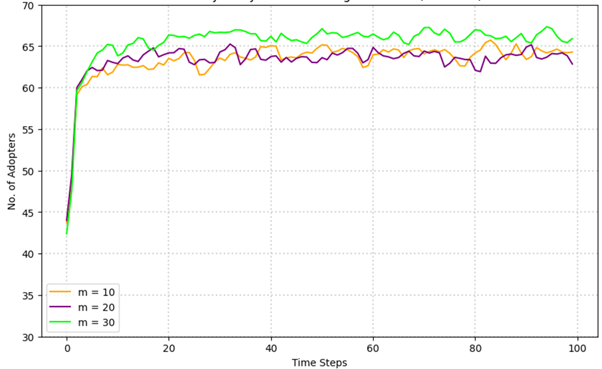
\includegraphics[width=0.45\textwidth]{1111.png} % Replace with the actual path
    \caption{Sensitivity analysis of marketing promotion input to the number of adopters (\( m = 10, 20, 30 \)).}
    \label{fig:marketing_promotion_sensitivity}
\end{figure}
Figure 5 reveals that as marketing promotion investment increases, the number of users adopting innovation, particularly during the early stages of diffusion. However, the advantages of higher marketing investment begin to diminish, which can be observed through the convergence of adoption rates, for \(m = 20\), and \(m = 10\), after \(T = 20\) time steps. Over time, adoption also increases among users with lower levels of marketing input, and the difference in the number of adopters among the three levels of promotion becomes less significant. This suggests that marketing’s influence on diffusion is primarily impactful at the start of process. This is intuitive, and consistent with real-life scenario, as marketing investments generally give initial boost to the sales of the product, but as time progresses, this effect diminishes. 
\subsubsection{Payoff Gains}
\begin{figure}[h]
    \centering
    % First Subfigure (Payoff Gains)
    \begin{subfigure}{0.45\textwidth}
        \centering
        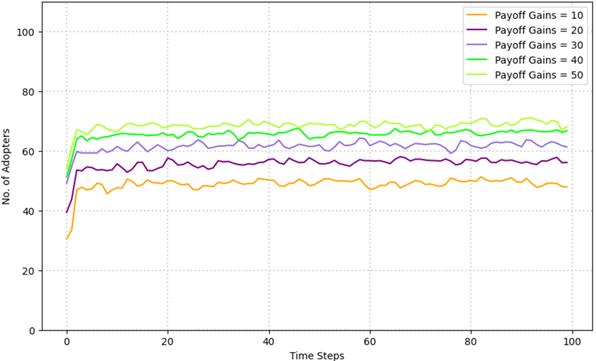
\includegraphics[width=\linewidth]{22222.png} % Replace with the actual path for the image
        \caption{}
        \label{fig:payoff_gains}
    \end{subfigure}
    % Space between images
    \hspace{0.05\textwidth}
    % Second Subfigure (Noise Sensitivity)
    \begin{subfigure}{0.45\textwidth}
        \centering
        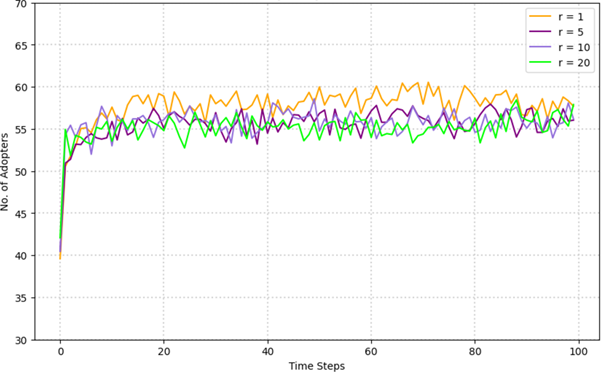
\includegraphics[width=\linewidth]{11111.png} % Replace with the actual path for the image
        \caption{}
        \label{fig:noise_sensitivity}
    \end{subfigure}
    \caption{(a) Analysis of adoption trends across different payoff gains. (b) Analysis of adoption trends across varying noise levels.}
    \label{fig:sensitivity_analysis}
\end{figure}
Payoff gain represents the benefit that a user receives from adopting an innovation, with respect to the status-quo state. To analyze the effect of payoff gains on the diffusion of digital solutions, we use the same model parameters outlined in Section 3.1.1. 

Figure 6(a) illustrates the impact of varying payoff gains, adjusted by changing the difference \( b - c \), on the number of adopters over time. As the payoff gain increases, we observe a corresponding rise in the adoption levels. Specifically, higher values of \( b - c \) result in a greater utility for adopting the innovation, incentivizing more users to adopt. This trend is evident in the graph, where higher payoff gains, such as \( b - c = 50 \), lead to a consistently larger number of adopters compared to lower payoff gains, like \( b - c = 10 \). The adoption rates stabilize relatively quickly, suggesting that once users perceive sufficient benefit from adoption, they are likely to maintain that choice. Thus, a more favorable payoff significantly enhances the attractiveness of the innovation, thus accelerating diffusion within the network.


\subsubsection{Noise Level}
In our model, noise is incorporated as a parameter that influences the likelihood of users adopting decisions from their neighbors, adding randomness to the decision-making process. The noise parameter, represented by \( r \), impacts the learning probability calculated by equation (7). High noise values reduce the importance of utility differences, making decisions more random. Figure 6(b) illustrates that higher noise levels initially lead to a rapid increase in innovation adoption, as randomness helps some users overcome their status quo bias. However, over time, higher noise results in lower and more volatile adoption rates, as observed in the case of \(r = 20\).

Noise makes decisions more random, but conservative users with high thresholds remain resistant, and matching probabilities further reinforce this resistance. In contrast, mutable users, who are more susceptible to shocks, are more easily influenced by the noise. Hence, high noise weakens the influence of network-driven behaviors and rather than encouraging adoption, higher noise levels create inconsistency and prevent stable adoption clusters from forming. This leads to lower overall diffusion, contrasting with traditional models where noise promotes independent adoption. The unique combination of personality-driven thresholds, utility-based decisions, and noise as random variation results in the observed diffusion patterns in figure 6(b). 
\subsection{Innovation Diffusion under Single-Agent Revision Process}

In this section, we examine innovation diffusion under a single-agent revision process. At discrete time intervals \( t = k/N \), with \( k \in \mathbb{N} \), a single agent is randomly chosen to potentially revise their decision to adopt or reject the innovation. The decision-learning process and model framework remain consistent with those described in Section 2.1.3. The model is simulated for 500 time steps to observe the long-term convergence of adoption rates, with results averaged over 50 runs to ensure robustness.

Previous literature \cite{kreindler2014rapid} has shown that, in the context of a single-agent revision process, given a positive noise level (\( r > 0 \)), if the payoff gain (\( \alpha = b - c \)) is sufficiently large (with the lower bound derived conditionally on the noise level), rapid diffusion occurs across all network structures. Specifically, for any graph \( G \), when \( \tilde{\mu}(\alpha, r) > 0 \), the expected waiting time until at least half of the population adopts the innovation, denoted by \( ET(\alpha, r, G) \), satisfies \( ET(\alpha, r, G) < \frac{1}{\tilde{\mu}} \). This inequality implies that with a sufficiently high payoff gain and a given noise level, the expected time for majority adoption is effectively bounded irrespective of the network's topology, which facilitates rapid diffusion.


\begin{figure}[h]
    \centering
    % First Subfigure
    \begin{subfigure}{0.32\textwidth}
        \centering
        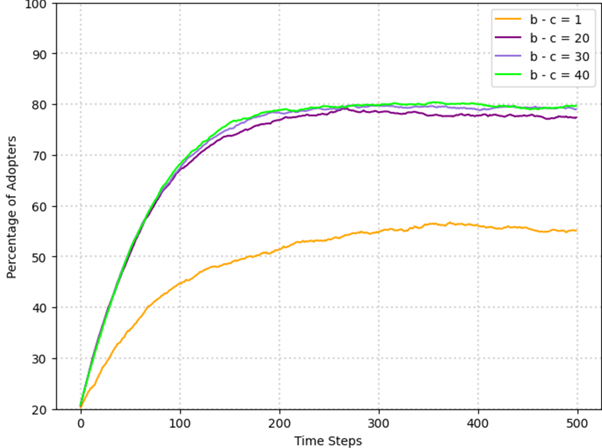
\includegraphics[width=\linewidth]{111111.png} % Replace with the actual path for the image
        \caption{}
        \label{fig:subfig1}
    \end{subfigure}
    \hfill
    % Second Subfigure
    \begin{subfigure}{0.32\textwidth}
        \centering
        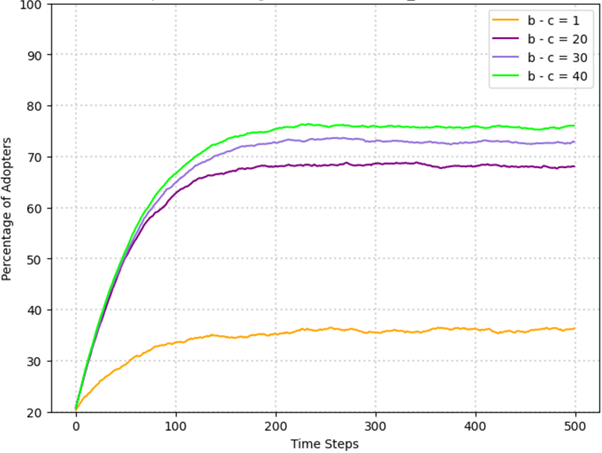
\includegraphics[width=\linewidth]{222222.png} % Replace with the actual path for the image
        \caption{}
        \label{fig:subfig2}
    \end{subfigure}
    \hfill
    % Third Subfigure
    \begin{subfigure}{0.32\textwidth}
        \centering
        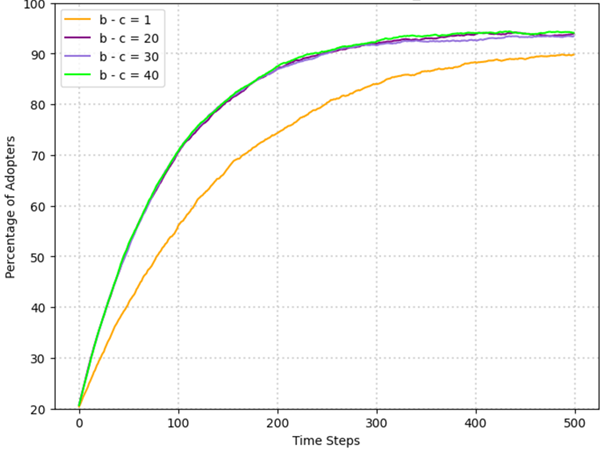
\includegraphics[width=\linewidth]{333333.png} % Replace with the actual path for the image
        \caption{}
        \label{fig:subfig3}
    \end{subfigure}
    \caption{Innovation Diffusion with Different Payoff Gains (a) Random Network. (b) Small-World Network. (c) Scale-Free Network.}
    \label{fig:adoption_trends}
\end{figure}

Figures 7 illustrate the diffusion dynamics under varying network structures—random, small-world, and scale-free networks, respectively with different levels of payoff gain. Across all network, significantly higher payoff gains, such as \(\alpha = 40 \), consistently result in faster and more stable adoption rates compared to lower gains like \( \alpha = 1 \). For instance, in all graphs, as \( \alpha \) reaches 40, we observe that the percentage of adopters quickly stabilizes at a high level. This trend aligns with the theoretical result that, given sufficient payoff gain, rapid diffusion can occur regardless of network topology. 

Sufficiently high payoff gain \( \alpha \) relative to the noise threshold significantly accelerates diffusion, reducing the waiting time for widespread adoption. In small-world networks, the local clustering initially limits adoption rates at lower payoff gains, as clusters of users are more resistant to innovation without sufficient incentive. However, as payoff gains increase significantly, these clusters overcome their decision thresholds, leading to a tipping point where the clustering accelerates diffusion. This effect results in a more rapid increase in adoption rates for small-world networks (relative to other structures), that initially had very less diffusion. The network's clustering thus becomes an advantage at higher payoff levels.  As observed in all three network types, increasing the payoff gain consistently accelerates adoption rates, suggesting that, beyond a certain threshold, the effect of network topology on diffusion speed becomes negligible. This finding implies that the expected waiting time until at least half the population adopts the innovation is effectively bounded for all the network topologies. 
\section{Conclusions}

In this research, we examined the diffusion dynamics of digital innovations in heterogeneous social networks, focusing on the influence of network effects, user diversity, and decision-making factors such as payoff gains, noise levels, firm marketing investments, and network structures. 

We found that scale-free networks enable the fastest adoption due to influential hubs, while small-world networks accelerate diffusion at higher payoff gains. Random networks require stronger incentives to achieve similar adoption rates. The research also revealed that User heterogeneity significantly influences diffusion. Our analysis also showed that both local and global network effects result in similar diffusion patterns across various social network structures. Additionally, the intensity of the network effect enhances the utility value of digital innovations and increases the duration of the diffusion process. Consistent with the findings of previous studies \cite{wei2019social, muller_network_2019}, our study reinforces the critical role of network structures in driving the diffusion of digital innovations. 

Furthermore, the results underscore the influence of user preferences and peer interactions on individual decision-making. Previous studies have also investigated the interplay between user preferences and decision-making processes through multi-agent models \cite{kickhofer2011income, kamel2019user}. These studies leverage the robustness of multi-agent frameworks to examine how user preferences impact decision-making, including in transportation contexts such as the adoption of shared autonomous vehicles. Finally, firm investments in marketing and promotional strategies during the early stages of market entry have been shown to significantly accelerate the speed and scale of initial diffusion, providing an effective way to boost adoption rates.

This study contributes to the literature by validating key driver variables behind the diffusion of digital applications. Network intensities and marketing play a crucial role in diffusion. Also, beyond a critical threshold of payoff gains, the influence of network topology diminishes, and rapid diffusion becomes feasible across all structures \cite{kreindler2014rapid}. The research has practical implications for designing marketing strategies and public policies aimed at accelerating the adoption of innovations.

\textit{\textbf{Limitations}}: While the model captures complex interactions within diverse network types, it assumes homogeneous payoff gains and uniform noise levels across agents, which may oversimplify real-world conditions. Additionally, the influence of external competing innovations and dynamic changes in user preferences were not considered, potentially limiting the model’s applicability to rapidly evolving digital markets. Moreover, the fixed structure of networks in our simulation does not account for the dynamic nature of social ties, which could impact the diffusion process over time.

\textit{\textbf{Future Work}}: Building on these limitations, future studies should explore adaptive network structures where connections evolve as adoption progresses. Examining scenarios with competing innovations could provide further insights into how users weigh multiple choices within their networks. Additionally, incorporating variable noise levels and dynamic payoff gains could enhance model robustness, making it more applicable to diverse real-world settings. Extending this research to analyze the impact of targeted marketing efforts on specific user types, such as highly influential nodes in scale-free networks, could offer firms more practical diffusion strategies.

\begin{thebibliography}{9}

\bibitem{amini2012alternative} 
Amini, M.; Wakolbinger, T.; Racer, M.; Nejad, M.G. Alternative supply chain production–sales policies for new product diffusion: An agent-based modeling and simulation approach. \textit{Eur. J. Oper. Res.} \textbf{2012}, \textit{216}, 301–311. [CrossRef]

\bibitem{rai2016agent} 
Rai, V.; Henry, A.D. Agent-based modelling of consumer energy choices. \textit{Nat. Clim. Chang.} \textbf{2016}, \textit{6}, 556–562. [CrossRef]

\bibitem{rogers_diffusion_2003}
Rogers, E.M. \textit{Diffusion of Innovations}; Free Press: New York, NY, USA, 2003.

\bibitem{granovetter_threshold_1978}
Granovetter, M. Threshold Models of Collective Behavior. \textit{Am. J. Sociol.} \textbf{1978}, \textit{83}, 1420–1443.

\bibitem{valente_network_1996}
Valente, T.W. Network Models of the Diffusion of Innovations; \textit{Comput. Math. Organ. Theory} \textbf{1996}, \textit{2}, 163–164.

\bibitem{young_diffusion_1996}
Young, H.P. The Economics of Convention. \textit{J. Econ. Perspect.} \textbf{1996}, \textit{10}, 105–122.

\bibitem{muller_network_2019}
Muller, E.; Peres, R. The Effect of Social Networks Structure on Innovation Performance: A Conceptual Framework. \textit{J. Mark.} \textbf{2019}, \textit{83}, 122–136.

\bibitem{song2018ecosystem}
Song, P.; Xue, L.; Rai, A.; Zhang, C. The ecosystem of software platforms: A study of asymmetric cross-side network effects and platform governance. \textit{MIS Q.} \textbf{2018}, \textit{42}, 121–142. [CrossRef]

\bibitem{young_individual_1998}
Young, H.P. Individual Strategy and Social Structure: An Evolutionary Theory of Institutions; Princeton University Press: Princeton, NJ, USA, 1998.

\bibitem{jiang2020review}
Jiang, G.; Shang, J.; Liu, W.; Feng, X.; Lei, J. Modeling the dynamics of online review life cycle: Role of social and economic moderations. \textit{Eur. J. Oper. Res.} \textbf{2020}, in press. [CrossRef]

\bibitem{yi2018management}
Yi, H.; Berry, F.S.; Chen, W. Management innovation and policy diffusion through leadership transfer networks: An agent network diffusion model. \textit{J. Public Adm. Res. Theory} \textbf{2018}, \textit{28}, 457–474. [CrossRef]

\bibitem{bryson2007agent}
Bryson, J.J.; Ando, Y.; Lehmann, H. Agent-based modelling as scientific method: A case study analysing primate social behaviour. \textit{Philos. Trans. R. Soc. B Biol. Sci.} \textbf{2007}, \textit{362}, 1685–1699. [CrossRef] [PubMed]

\bibitem{joseph2020organizational}
Joseph, J.; Gaba, V. Organizational Structure, Information Processing, and Decision-Making: A Retrospective and Road Map for Research. \textit{Acad. Manag. Ann.} \textbf{2020}, \textit{14}, 267–302. [CrossRef]

\bibitem{hann2007overcoming}
Hann, I.H.; Hui, K.L.; Lee, S.Y.T.; Png, I.P.L. Overcoming online information privacy concerns: An information-processing theory approach. \textit{J. Manag. Inf. Syst.} \textbf{2007}, \textit{24}, 13–42. [CrossRef]

\bibitem{ozkan2016evolutionary}
Ozkan-Canbolat, E.; Beraha, A.; Bas, A. Application of evolutionary game theory to strategic innovation. \textit{Procedia Soc. Behav. Sci.} \textbf{2016}, \textit{235}, 685–693. [CrossRef]

\bibitem{zhang2019competitive}
Zhang, R.; Sun, B. A competitive dynamics perspective on evolutionary game theory, agent-based modeling, and innovation in high-tech firms. \textit{Manag. Decis.} \textbf{2019}. [CrossRef]

\bibitem{kreindler2014rapid}
Kreindler, G.E.; Young, H.P. Rapid Innovation Diffusion in Social Networks. \textit{Proc. Natl. Acad. Sci. USA} \textbf{2014}, \textit{111}, 10881–10888. [CrossRef]

\bibitem{wei2019social}
Wei, X.; Chen, W. How does a firm’s previous social network position affect innovation? Evidence from Chinese listed companies. \textit{Sustainability} \textbf{2019}, \textit{11}, 1191. [CrossRef]

\bibitem{kickhofer2011income}
Kickhöfer, B.; Grether, D.; Nagel, K. Income-contingent user preferences in policy evaluation: Application and discussion based on multi-agent transport simulations. \textit{Transportation} \textbf{2011}, \textit{38}, 849. [CrossRef]

\bibitem{kamel2019user}
Kamel, J.; Vosooghi, R.; Puchinger, J.; Ksontini, F.; Sirin, G. Exploring the impact of user preferences on shared autonomous vehicle modal split: A multi-agent simulation approach. \textit{Transp. Res. Procedia} \textbf{2019}, \textit{37}, 115–122. [CrossRef]

\end{thebibliography}

\end{document}